% ===================== 第 2 章 =====================
\section{方法总览：一个记忆内核与三根支柱}

Poliscope 回答的问题是：\textbf{一套多智能体研究系统要满足什么组织结构，才能让「被质疑过的结论」可追溯、让少数意见活下来、让过程材料冒充不了证据。}本章先给出整体轮廓，后续章节再逐层展开机制。

\subsection{方法定位：从 MemoBrain 到 EpistemoBrain，再到 Poliscope}

定位分两步说清楚。

\textbf{第一步，EpistemoBrain 是什么。}它\emph{不是}整个 Poliscope，也不是「N 个 MemoBrain 的堆叠」，而是 MemoBrain 执行记忆机制从单智能体到多智能体的推广——一套关于\textbf{多智能体记忆压缩}的方法，管理三层记忆并重新定义三个压缩操作。它不投票、不产出科研判断、不代表任何学术立场。

\textbf{第二步，它怎么进入 Poliscope。}EpistemoBrain 是本项目的\textbf{核心算法}，由三部分构成：集体执行记忆、异议保真记忆操作、盲点驱动调度。它本身可以独立存在，也可以移植到别的多智能体场景；而在 Poliscope 里，它被专门适配进议会的决策框架——为什么要适配、以及扩展了哪五处，见下一节。Poliscope 还有另外两块\textbf{不属于} EpistemoBrain 的设计：决定「谁在研究、如何互相质询」的七人科学议会（第 4 章），和决定「什么算证据、怎么强制」的双图证据治理（第 6、7 章）。

MemoBrain 为\textbf{单个}推理智能体提供执行记忆：一张依赖感知的推理步骤图，用 \code{Flush} 剪掉无效路径、\code{Fold} 压缩已完成的子轨迹、\code{Recall} 在固定 token 预算内重建高显著上下文。这三个操作都建立在同一个前提上——\textbf{一个智能体自己检索、自己推理、自己压缩自己的过去}。

把这一个智能体换成一个多智能体集体，记忆的分析单位就从\textbf{私人轨迹}变成\textbf{集体共享认知状态}，三个原生操作也随之改变含义：

\begin{itemize}[leftmargin=1.6em, itemsep=3pt]
\item \textbf{Flush $\rightarrow$ Quarantine}：被反驳的主张不消失，改为保留状态历史——谁反驳的、缺什么证据、满足什么条件可以复活（第 5 章）。
\item \textbf{Fold $\rightarrow$ Dialectical Fold}：争议只在正反双方最强立场、枢纽变量与证伪条件都被保留之后才压缩。
\item \textbf{Recall $\rightarrow$ Perspective Recall}：每个成员召回的是共享图的一个角色专属投影，而不是同一份无差别摘要。
\end{itemize}

这个推广还带来一条单智能体场景不会出现的硬约束：\textbf{集体的记忆要被「不是写它的人」读到}。因此过程材料与正式结论必须分成两张图——一个成员的瞬时猜测，绝不能悄悄升级成其他人当作已核实的结论。这条约束直接决定了第 3 章的架构形态。图~\ref{fig:generalization} 给出完整对照。

机制本身不指定任何领域：它只依赖三样由场景注入的东西——\textbf{角色规格}（成员数量与各自专长）、\textbf{准入策略}（什么材料可以进入共享图、如何分级）、\textbf{共享图 schema}（有哪些节点类型与边类型）。Poliscope 填入的是科学争议审查这一组取值。

\begin{figure}[ht]
\centering
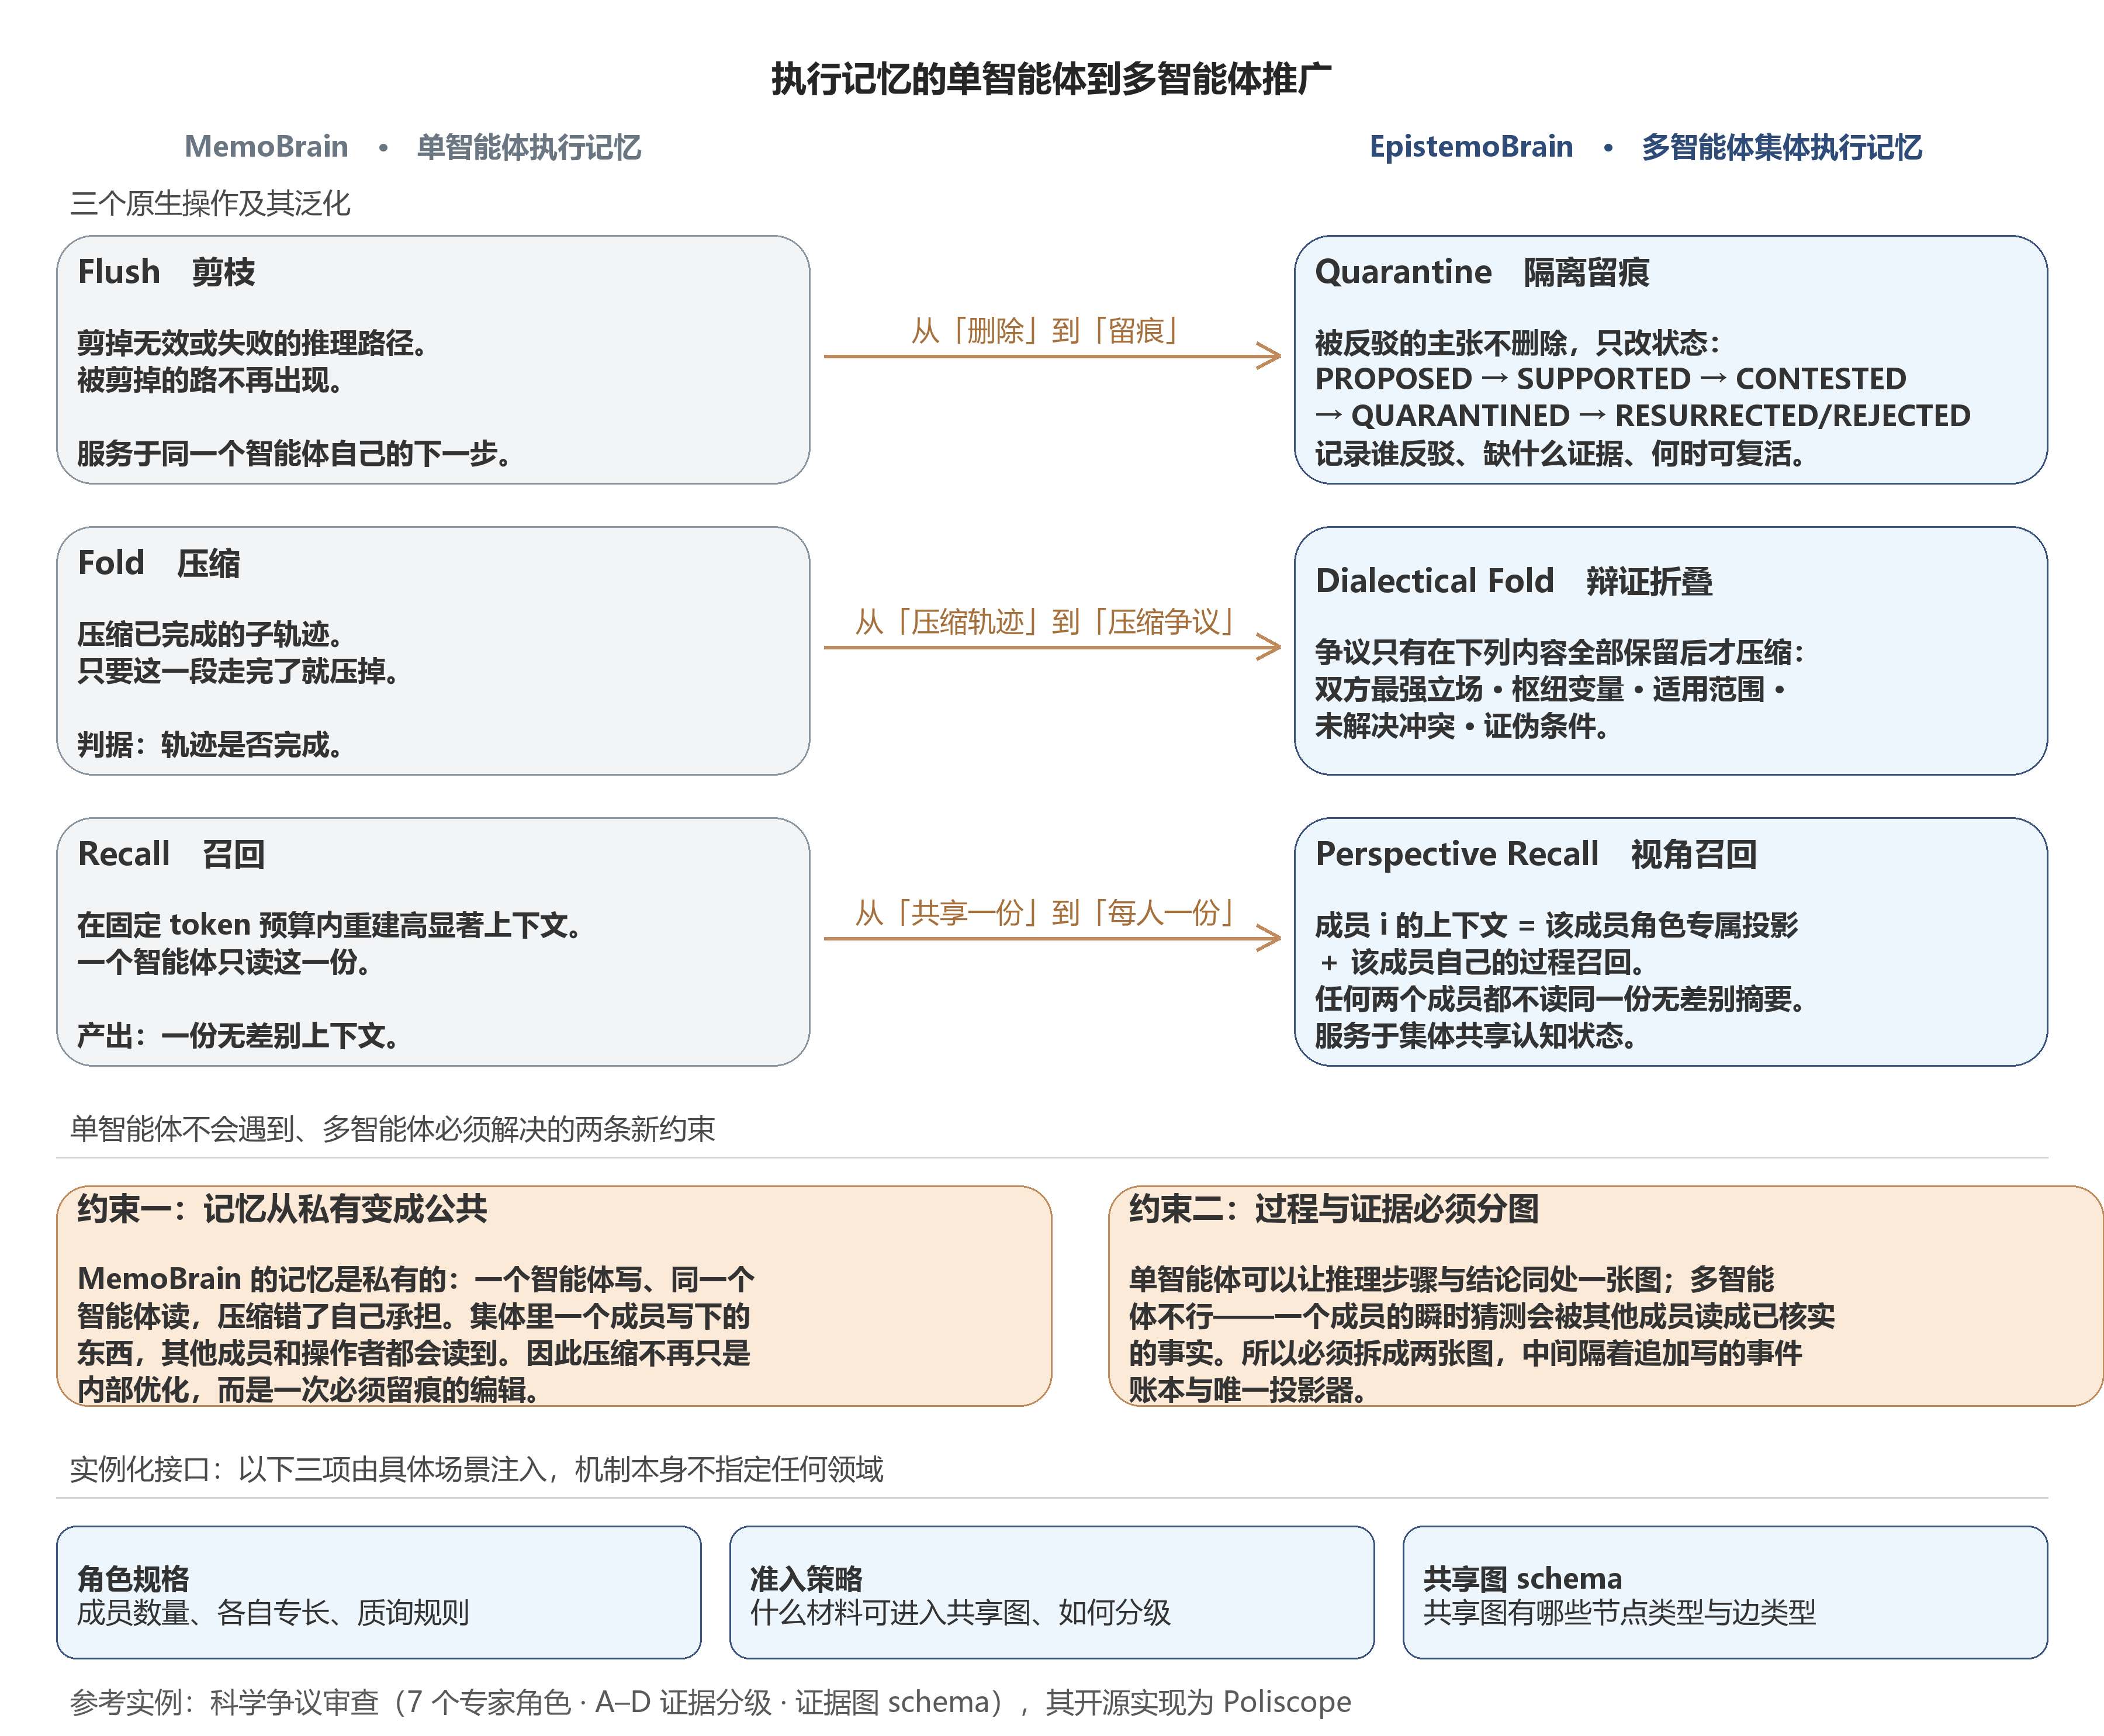
\includegraphics[width=\linewidth]{figures/memobrain-generalization.png}
\caption{执行记忆从单智能体到多智能体的推广。左列为 MemoBrain 的三个原生操作及其单智能体语义，右列为泛化后的操作与多智能体语义，中列标注推动这次转化的判据变化。中部两条约束只在多智能体场景出现：记忆由私有变为公共，过程与证据必须分图。底部为实例化接口——机制本身不指定领域，角色规格、准入策略与共享图 schema 由具体场景注入；科学争议审查是本文使用的参考实例，Poliscope 是它的开源实现。}
\label{fig:generalization}
\end{figure}

\subsection{适配：从单智能体记忆到议会的决策框架}

换的不只是调用方。MemoBrain 原本针对的是「一个 Agent、一个明确目标、逐步淘汰错误路线并保留正确推理骨架」；而议会面对的是「多个科学家围绕一个存在争议、可能没有唯一答案的问题长期协作与对抗」。两者之间有三个本质区别。

\begin{enumerate}[leftmargin=1.6em, itemsep=4pt]
\item \textbf{科研中的「失败观点」可能非常重要。}普通任务里，一条被证明无效的推理路线可以 \code{Flush}；但在科研中，一个当前不被支持的观点可能是有价值的少数派假设、在特殊人群中成立的边界条件、暂时缺少数据的理论解释，或以后会被新证据复活的研究方向。所以不能简单删除。
\item \textbf{科研争议不能被压缩成单一摘要。}普通 \code{Fold} 会把一段辩论总结成「多数证据支持 X」，而这恰恰丢失了最重要的信息：哪些研究不支持 X、不支持的原因是什么、样本或测量口径有什么差异、少数意见在哪些条件下可能成立。压缩一旦消灭异议，系统就会产生\textbf{共识幻觉}。
\item \textbf{不同的科学家需要不同的记忆视图。}因果推断专家要先看到识别策略、混杂变量、反向因果与自然实验；测量专家要先看到变量操作化、量表效度、数据来源与构念漂移。如果所有席位读取完全相同的压缩上下文，多智能体很快就会观点同质化。
\end{enumerate}

这三个区别决定了 EpistemoBrain 相对 MemoBrain 的\textbf{五个扩展}——它们不是功能堆叠，而是依次咬合的：集体记忆要留住争议，留住争议才谈得上识别盲点，识别出盲点才知道该调度谁。

\begin{table}[ht]
\centering\small
\caption{EpistemoBrain 相对 MemoBrain 的五个扩展}
\label{tab:extend}
\begin{tabularx}{\linewidth}{@{}L{2.9cm} L{3.1cm} X@{}}
\toprule
\rowcolor{accent}
\tblhead 扩展 & \tblhead 对应操作 & \tblhead 解决的区别 \\
\midrule
异议保真压缩 & \code{Dialectical Fold} & 争议须在双方最强立场、枢纽变量与证伪条件全部保留之后才压缩（区别 2）\\
证据隔离 & \code{Quarantine} & 被反驳的主张不删除，保留反驳者、缺失证据与复活条件（区别 1）\\
认知分叉 & \code{Fork} / \code{Merge} / \code{Resurrect} & 证据无法区分解释时保留平行路径；新证据满足条件时复活旧假设（区别 1）\\
角色化召回 & \code{Perspective Recall} & 按 \code{Context\_i = ProcessRecall\_i + EvidenceProjection\_i} 计算，七席读到的不是同一份摘要（区别 3）\\
盲点驱动调度 & 盲点悬赏与认识论路由 & 由证据图暴露的缺口决定下一步查什么、由谁查（第 5.3 节）\\
\bottomrule
\end{tabularx}
\end{table}

适配的落点是三层记忆的重新划分（第 5.1 节）：第一层 \code{Private Brain} 直接复用 MemoBrain 的 \code{init\_memory()}、\code{memorize()}、\code{recall()}、token 预算控制与轨迹 Fold，只服务该席位自己，不被其他席位读取；第二层\textbf{集体执行记忆}是本项目的主要创新，它不存聊天记录，只存结构化的认知事件——谁提出了什么、谁攻击了什么、哪些争议尚未解决；第三层争议证据地图则完全移出记忆层，交给双图治理（第 6 章）。记忆层对证据图\emph{没有任何写入权}。

适配的收益是双向的。一方面，议会由此获得了在有限预算内维持长程一致性的机制；另一方面，「记忆由私有变为公共」这条新约束反过来塑造了议会本身的形态——正因为一次压缩的结果会被没写过它的同伴读到，压缩才必须留痕，「过程与证据分图」才成为不可省略的架构决策，而不是可选的工程优化。

\subsection{三根支柱}

整套方法由三根支柱构成，分别对应「谁在研究」「靠什么记得」「什么算证据」。

\begin{enumerate}[leftmargin=1.6em, itemsep=5pt]
\item \textbf{集体协议（Collective Protocol）}回答「谁在研究」。Poliscope 在这一层填入的取值是七人科学议会：七个固定角色各有独立规格、私人状态、私人记忆与证据排序权重，按八阶段协议用结构化动作互相质询。多视角不靠人多，靠每个视角被制度化地挑战。详见第 4 章。
\item \textbf{EpistemoBrain（记忆内核）}回答「靠什么记得」。它把 MemoBrain 的单智能体执行记忆推广到多智能体，管理私人记忆、集体执行记忆与证据图三层，并重新定义三个压缩操作。三层之间形成「过程产生证据、证据暴露盲点、盲点驱动下一轮调查」的闭环——集体记忆不是存档柜，它参与决定下一轮查什么。详见本章「方法定位」与「适配」两节，以及第 5 章。
\item \textbf{双图证据治理（Dual-Graph Governance）}回答「什么算证据」。过程图与证据图物理分离，中间隔着追加写的事件账本、六阶段证据门和唯一投影器。详见第 6、7 章。
\end{enumerate}

\subsection{一次研究的认识论循环}

三根支柱在一次真实任务中串成一条八阶段循环（图~\ref{fig:loop}）。每个阶段都对应一个它专门防止的失败：预承诺防锚定，专业取证防空谈，证据交换防重复阅读，交叉质询防隐藏假设，盲点悬赏把无人触碰的缺口显式化，联合建模防多数票冒充共识，最终复判防信念漂移后无人记账，报告阶段只做组装、不再产生新判断。

\begin{figure}[ht]
\centering
\resizebox{\linewidth}{!}{%
\begin{tikzpicture}[node distance=1.0mm and 3.5mm]
  \node[nda] (p1) {1 独立预承诺};
  \node[nd, right=of p1] (p2) {2 专业取证};
  \node[nd, right=of p2] (p3) {3 证据交换};
  \node[nd, right=of p3] (p4) {4 交叉质询};
  \node[nda, below=of p4] (p5) {5 盲点悬赏};
  \node[nd, left=of p5] (p6) {6 联合建模};
  \node[nd, left=of p6] (p7) {7 最终复判};
  \node[ndd, left=of p7] (p8) {8 报告组装};
  \draw[flow] (p1)--(p2); \draw[flow] (p2)--(p3); \draw[flow] (p3)--(p4);
  \draw[flow] (p4)--(p5); \draw[flow] (p5)--(p6); \draw[flow] (p6)--(p7); \draw[flow] (p7)--(p8);
  \draw[flowg] (p5.south) to[bend right=22] node[lbl,pos=0.5]{缺口生成新调查任务} (p2.south);
\end{tikzpicture}}
\caption{EpistemoBrain 认识论循环：蓝色为两个「判断封存」关键点；第 5 阶段的盲点可回流到第 2 阶段形成增量调查。}
\label{fig:loop}
\end{figure}

\subsection{三条认识论硬约束}

\begin{mechbox}
\boxtag{\color{ink2}不投票}
禁止以多数投票裁决科研真理。即使多数席位支持，只要存在未解决的致命质询或缺乏证据引用，共识就被阻断；最终输出必须同时写出多数判断、具名异议、真正分歧点与解决分歧所需证据（第 4.4 节）。
\end{mechbox}

\begin{mechbox}
\boxtag{\color{ink2}不匿名删除异议}
被反驳、隔离或折叠的观点不做物理删除，只改状态并保留谱系；辩证折叠要求正反双方字段齐备，缺一方就拒绝折叠（第 6.7 节）。
\end{mechbox}

\begin{mechbox}
\boxtag{\color{ink2}不把过程当证据}
任何参与成员都没有证据图写权限；正式修改先写事件账本，由唯一投影器过证据门后落图。这条约束在数据库角色权限层强制，而非依赖代码自律（第 6.5、11.7 节）。
\end{mechbox}

\subsection{与两条主流路线的边界}

Deep Research 优化「读得全」，固定多智能体辩论优化「吵得充分」，EpistemoBrain 优化「被质疑过的结论仍然可追溯」。表~\ref{tab:compare} 给出机制层面的对照，后文每一行都有对应章节落地。

\begin{table}[ht]
\centering\small
\caption{EpistemoBrain 与两类常见研究智能体的机制对照}
\label{tab:compare}
\begin{tabularx}{\linewidth}{@{}L{2.5cm} XXX@{}}
\toprule
\rowcolor{accent}
\tblhead 维度 & \tblhead Deep Research & \tblhead 固定多智能体辩论 & \tblhead EpistemoBrain \\
\midrule
多视角来源 & 单 Agent 换提示词 & 多 Agent 自由发言 & 7 席独立角色规格，结构化动作质询 \\
异议去向 & 并入总结 & 多数意见胜出 & 具名异议证书，永久留图 \\
记忆机制 & 上下文窗口 & 彼此独立、无共享 & 三层记忆，集体记忆调度下一轮 \\
证据标准 & 引用存在即可 & 引用存在即可 & 六阶段证据门 + 因果越级拦截 \\
证据写权限 & 无此概念 & 无此概念 & 数据库层唯一投影器 \\
最终产物 & 流畅综述 & 辩论记录 & 结论与局限并排的可审计证据地图 \\
\bottomrule
\end{tabularx}
\end{table}
